% Drawing 156-6/04-6 -- folder 156-6, batch 04, archive page 79 (PDF page 80).
% Transcription: schéma d'implications : doubles flèches de At $9_{\Sigma}$ vers At 9 et vers At 12, de At 12 vers At 10 et vers « At 11' pour $\widetilde{F}$ fini », de At 11 vers At 11', de « At 11 pour $F = \operatorname{Sup} F_i$ quelc. » vers « At 11 pour $F = \operatorname{Sup} F_i$ fini », et de At 11' vers « At 11' pour $\widetilde{F}$ fini ». Une équivalence avec « At 11 » à la fin de la dernière ligne est biffée, ainsi qu'un signe dans la marge gauche
% Kind: diagram of implications between axioms At 9 ... At 12. Method 2 (schematic redraw from the facsimile). Status: ok.
% Notes: Double arrows (drawn single): At 9_Sigma => At 9 and => At 12 (downwards); At 12 => At 10 and, by a bent arrow, => "At 11' pour F~ fini"; At 11 => At 11'; At 11 <=> "At 11 pour F = Sup F_i quelc.", which => "At 11 pour F = Sup F_i fini"; At 11' <=> "At 11 pour F = Sup F_i fini" (overinked, not struck: the transcription's array reads this equivalence, so it is now drawn in ink); At 11' => "At 11' pour F~ fini". Omitted as struck: the equivalence "<=> At 11" at the end of the last line and the sign in the left margin. Issue 128, 2026-11-09: struck material left out after a fresh check of the facsimile (struck-out material is not drawn). Redrawn 2026-11-09 (issue 128): to check again.
% Coordinates: 1 unit = 1 mm = 1/100 of the crop width (bbox in page fractions: [0.12, 0.1, 0.95, 0.23]).
% Redrawn by Claude (claude-opus-5-5), issue #73, 2026-11-07; not checked by a human; not compiled (no TeX in the session).
% Rights: reproduces part of the work -- behind RENDER_TRANSCRIPTS, never published by itself.
\documentclass[tikz,border=3pt]{standalone}
\usepackage{amsmath,amssymb}
\usetikzlibrary{patterns,arrows.meta}
\tikzset{pencil/.style={black!45}, struck/.style={black!35}, mark/.style={circle,draw,inner sep=1.3pt}, pt/.style={circle,fill,inner sep=0.9pt}, opt/.style={circle,draw,fill=white,inner sep=1.1pt}}
\begin{document}
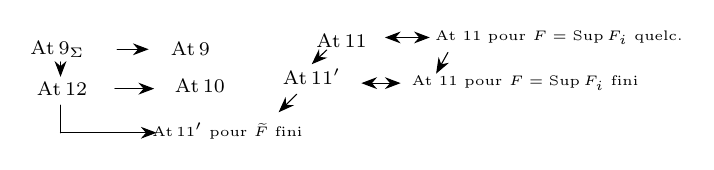
\begin{tikzpicture}[x=1mm,y=1mm,line cap=round,line join=round,font=\scriptsize]
\node[inner sep=1pt] at (30.4,-6.9) {\scriptsize $\mathrm{At}\,9_\Sigma$};
\node[inner sep=1pt] at (47.3,-6.9) {\scriptsize $\mathrm{At}\,9$};
\node[inner sep=1pt] at (31,-11.9) {\scriptsize $\mathrm{At}\,12$};
\node[inner sep=1pt] at (48.5,-11.5) {\scriptsize $\mathrm{At}\,10$};
\node[inner sep=1pt] at (52,-17.3) {\tiny $\mathrm{At}\,11'$ pour $\widetilde F$ fini};
\node[inner sep=1pt] at (66.5,-5.8) {\scriptsize $\mathrm{At}\,11$};
\node[inner sep=1pt] at (62.7,-10.4) {\scriptsize $\mathrm{At}\,11'$};
\node[inner sep=1pt,anchor=west] at (78,-5.4) {\tiny At 11 pour $F=\mathrm{Sup}\,F_i$ quelc.};
\node[inner sep=1pt,anchor=west] at (75,-11.2) {\tiny At 11 pour $F=\mathrm{Sup}\,F_i$ fini};
\draw[-{Stealth[length=2mm]}] (38,-6.9) -- (42,-6.9);
\draw[-{Stealth[length=2mm]}] (30.8,-8.5) -- (30.8,-10.4);
\draw[-{Stealth[length=2mm]}] (37.7,-11.9) -- (42.7,-11.9);
\draw (30.8,-14) -- (30.8,-17.5);
\draw[-{Stealth[length=2mm]}] (30.8,-17.5) -- (43,-17.5);
\draw[-{Stealth[length=2mm]}] (64.6,-7) -- (62.7,-8.8);
\draw[{Stealth[length=2mm]}-{Stealth[length=2mm]}] (72,-5.4) -- (77.7,-5.4);
\draw[-{Stealth[length=2mm]}] (80,-7.3) -- (78.5,-10);
\draw[-{Stealth[length=2mm]}] (60.8,-12.6) -- (58.5,-14.9);
\draw[{Stealth[length=2mm]}-{Stealth[length=2mm]}] (69,-11.2) -- (74,-11.2);
\end{tikzpicture}
\end{document}
